%!TEX root = ../cursus_fys6.tex
\chapter{Tweedimensionale bewegingen}

Als we in een vlak bewegen, hebben we te maken met een tweedimensionale beweging. 
Om ze te beschrijven voeren we nu een referentiestelsel met twee assen in. In de regel kiezen we een cartesiaans assenstelsel.  Door de co\"ordinaten $(x,y)$ van een punt dat het bewegende object voorstelt te geven, kunnen we de positie beschrijven. We kunnen echter ook een vector gebruiken.
\begin{figure}[h]
\centering
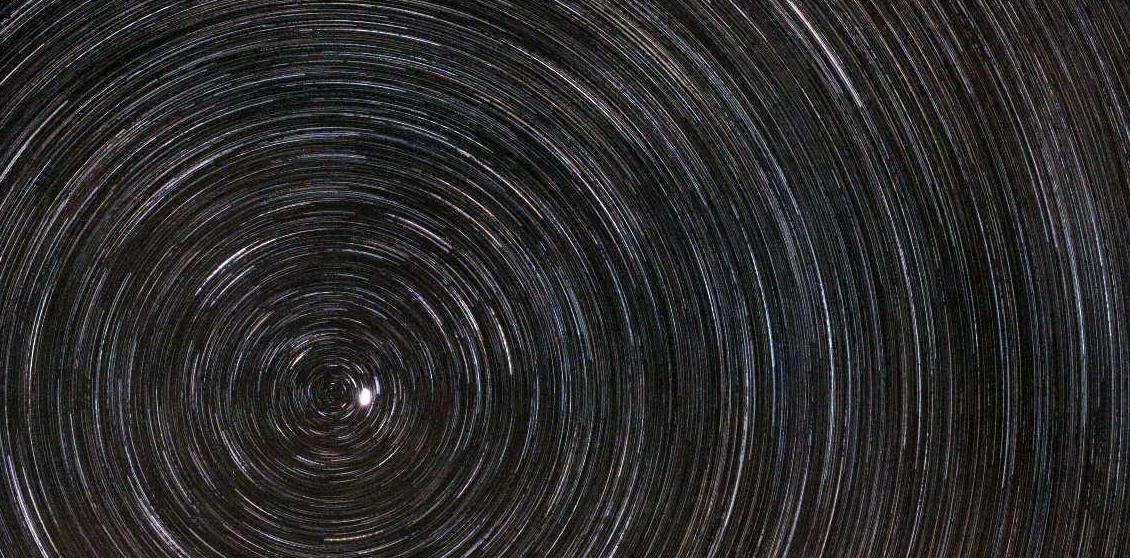
\includegraphics[width=.7\textwidth]{sterrentrajecten}
\caption{Sterrentrajecten aan de hemel}
\end{figure}
Omdat we om de snelheid van het object te kunnen beschrijven niet voldoende hebben aan alleen maar de grootte maar ook nood hebben aan een richting, maken we nu expliciet gebruik van vectoren en hun geschikte eigenschappen. Naast een nieuwe as voor de extra dimensie is het gebruik van vectoren de enige aanpassing die we aan ons formalisme van de kinematica moeten doen om bewegingen in twee dimensies te kunnen beschrijven.

\section{Onafhankelijkheidsbeginsel}

Stel je voor dat het heel mooi weer is. Zo van dat weer waar de hemel hemelsblauw is, er geen wolken aan de lucht zijn, de zon aan de hemel schittert en je niets liever doet dan een frisse neus halen. In zo'n weer zouden we diep in en uit ademen. Oh ja, detail, stel je ook voor dat er \emph{geen}\footnote{Begrijpelijk zou je kunnen opwerpen dat het nogal moeilijk is om frisse lucht die er niet is, in te ademen.} lucht is. Stel je bovendien voor dat je in het kraaiennest van een piratenschip zit. Het schip vaart met een gestadige, grote en constante snelheid over het zee-oppervlak dat geen enkele rimpeling vertoont. Golven zijn er niet\footnote{Ook hier zou je kunnen opperen dat een zee zonder golven niet echt een zee is.}. Stel je ook voor dat je een nogal zware kogel naar je uitkijkpost hebt meegenomen\footnote{Tja, in een gedachte-experiment zoals dit is veel mogelijk.}. Als je nu deze kogel laat vallen, met zicht op het achtersteven van het schip, dan \ldots dan valt hij natuurlijk regelrecht naar beneden op het hoofd van de kapitein die aan de voet van de mast staat en waarvoor me het arsenaal bijvoeglijke naamwoorden om zijn onuitstaanbaarheid te kunnen uitdrukken, even ontbreekt. Stel je nu ook voor dat zogezegd door de snelheid van het schip de kogel \emph{achter} het schip zou terechtkomen\footnote{Jawel, er zijn er onder ons die zich dat voorstellen} \ldots, dan zouden in een snel rijdende trein de valiezen die je op het rek legt zich met een enorme snelheid naar de achterkant van de wagon begeven, de kaarten die je wilt afleggen eveneens dezelfde plaats opzoeken i.p.v. netjes op de  aflegstapel te blijven liggen en dan zou de dame van de koffiebar enig kuiswerk hebben met de koffie die een ware ravage zou aanrichten \ldots 
\begin{figure}[h]
\centering
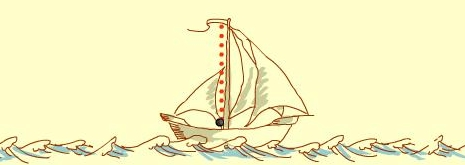
\includegraphics[height=2.3cm]{galileo_projectiles1} 
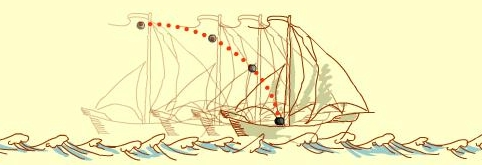
\includegraphics[height=2.3cm]{galileo_projectiles2} 
\caption{Dezelfde beweging van een kogel gezien door een waarnemer op het schip en een waarnemer buiten het schip.}
\end{figure}
Conclusie? Wel, de conclusie is enerzijds dat door de traagheid de kogel tijdens de val zijn snelheid vooruit, volgens de beweging van het schip, behoudt en recht op de kapitein terechtkomt en anderzijds dat de tijd die de kogel nodig heeft om in het luchtledige op de grond terecht te komen, onafhankelijk is van de snelheid die de kogel al dan niet meekrijgt in horizontale richting. De beweging van de kogel is immers voor iemand op het schip een verticale valbeweging en voor een buitenstaander een horizontale worp. Maar in beide gevallen gaat het om dezelfde beweging en dus ook over dezelfde benodigde tijd.\footnote{Mooie animatie: \url{http://www.pbs.org/wgbh/nova/galileo/expe_flash_2.html}}

\section{Enkele begrippen}

\subsection{Plaats, verplaatsing, afgelegde weg}

Om aan een vectori\"ele snelheid te komen, voeren we een plaatsvector $\vec{r}$ in. Deze kan van de tijd afhangen en kunnen we met behulp van de eenheidsvectoren $\vec{e}_x$ en $\vec{e}_y$ schrijven als
\begin{equation*}
 \vec{r}=x\cdot\vec{e}_x+y\cdot\vec{e}_y.
\end{equation*}
De tijdsafhankelijkheid kunnen we expliciet weergeven door $x(t)$ en $y(t)$ te gebruiken i.p.v. $x$ en $y$. De functies $x(t)$ en $y(t)$ noemen we de \emph{co\"ordinaat\-functies}. Door de plaats met een vector te beschrijven, kunnen we het begrip verplaatsing $\Delta x$ ook gemakkelijk en analoog uitbreiden naar twee dimensies. De verplaatsing
\begin{equation*}
\Delta\vec{r}=\vec{r}_2-\vec{r}_1
\end{equation*}
is nu immers ook een vector die naast de afstand in vogelvlucht tussen twee punten, ook ge\"ori\"enteerd is. Het is natuurlijk belangrijk in welke richting die afstand wordt afgelegd.
\begin{figure}[h]
\centering
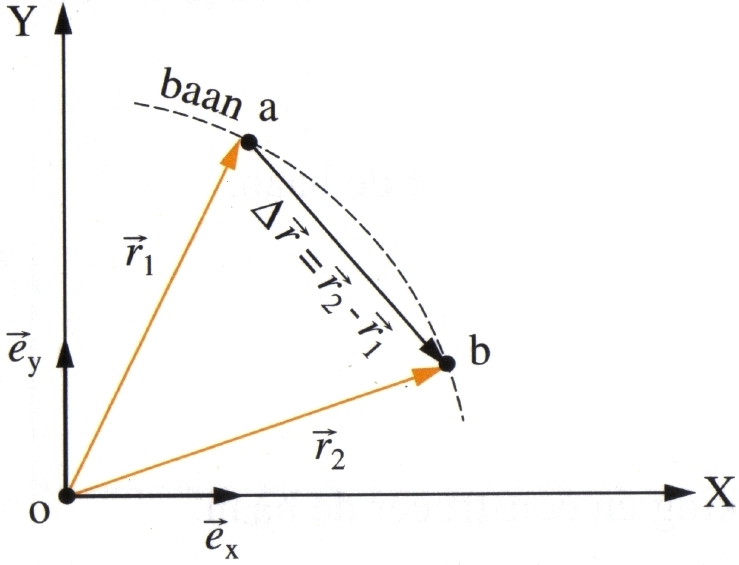
\includegraphics[width=0.4\textwidth]{plaatsvector}
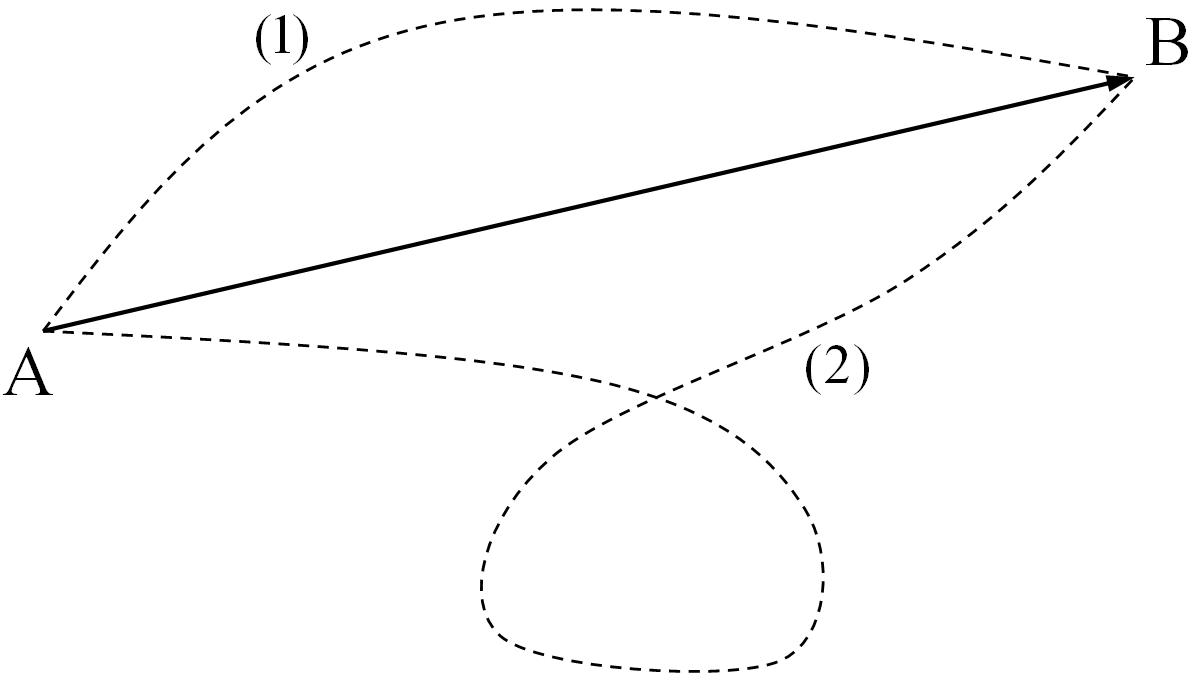
\includegraphics[width=0.4\textwidth]{afgelegdeweg_verplaatsing}
\caption{Het verschil tussen afgelegde weg en verplaatsing}
\end{figure}
Merk op dat de begrippen verplaatsing en afgelegde weg niet hetzelfde zijn. De afgelegde weg hangt af van de gevolgde baan en is de totale afgelegde afstand terwijl de verplaatsing enkel van begin- en eindpunt afhangt en een vectorgrootheid is.

Naast de co\"ordinaatfuncties $x(t)$ en $y(t)$ is er ook de vergelijking van de baan $y(x)$. We bekomen deze door de tijd uit de co\"ordinaatfuncties te elimineren\footnote{Dit komt neer op de inverse $t(x)$ van $x(t)$ te vinden en deze te substitueren in $y(t)$. Dus $y(x)=y(t(x))$.}. De grafiek van deze baanvergelijking geeft ons het beeld van de baan maar zegt niets over de snelheid waarmee het object over deze baan beweegt. Daarvoor hebben we de afhankelijkheid van de tijd nodig.

\subsection{Snelheid}

%\begin{wrapfigure}[9]{R}{0.35\textwidth}
%\centering
%\includegraphics[width=0.34\textwidth]{snelheidsvector}
%\end{wrapfigure}
Analoog aan de snelheid in \'e\'en dimensie, kunnen we in meerdere dimensies de snelheid defini\"eren als de afgeleide -- nu van de plaatsvector. De snelheid is dan opnieuw een vector:\footnote{De definitie van een afgeleide van een vector is evenzeer met een limiet. We maken gebruik van de uitdrukkingen $\vec{r}(t+\Delta t)=x(t+\Delta t)\vec{e}_x+y(t+\Delta t)\vec{e}_y$ en $\vec{r}(t)=x(t)\vec{e}_x+y(t)\vec{e}_y$.\begin{eqnarray*}
\vec{v}=\frac{d\vec{r}}{dt}&=&\lim_{\Delta t\to 0}\frac{\vec{r}(t+\Delta t)-\vec{r}(t)}{\Delta t}\\
&=&\lim_{\Delta t\to 0}\frac{[x(t+\Delta t)\vec{e}_x+y(t+\Delta t)\vec{e}_y]-[x(t)\vec{e}_x+y(t)\vec{e}_y]}{\Delta t}\\
&=&\lim_{\Delta t\to 0}\frac{[x(t+\Delta t)-x(t)]\vec{e}_x+[y(t+\Delta t)-y(t)]\vec{e}_y}{\Delta t}\\
&=&\lim_{\Delta t\to 0}\left(\frac{x(t+\Delta t)-x(t)}{\Delta t}\right)\vec{e}_x+\lim_{\Delta t\to 0}\left(\frac{y(t+\Delta t)-y(t)}{\Delta t}\right)\vec{e}_y\\
&=&\frac{dx}{dt}\vec{e}_x+\frac{dy}{dt}\vec{e}_y%\\&=&v_x\vec{e}_x+v_y\vec{e}_y
\end{eqnarray*}}
\begin{eqnarray*}
\vec{v}=\frac{d\vec{r}}{dt}=\frac{d}{dt}\left(x\cdot\vec{e}_x+y\cdot\vec{e}_y\right)=\frac{dx}{dt}\vec{e}_x+\frac{dy}{dt}\vec{e}_y%=v_x\vec{e}_x+v_y\vec{e}_y
\end{eqnarray*}
De eenheidsvectoren $\vec{e}_x$ en $\vec{e}_y$ veranderen niet in de tijd zodat we die buiten de afgeleide hebben kunnen brengen. We zien dat de snelheidsvector dus te ontbinden is in componenten waarbij de componenten gewoonweg de snelheden van de afzonderlijke co\"ordinaten zijn. 
\begin{eqnarray*}
\vec{v}=v_x\vec{e}_x+v_y\vec{e}_y\quad\mathrm{met}\quad v_x=\frac{dx}{dt},\,v_y=\frac{dy}{dt}
\end{eqnarray*}

%\begin{figure}[h]
%\centering
%%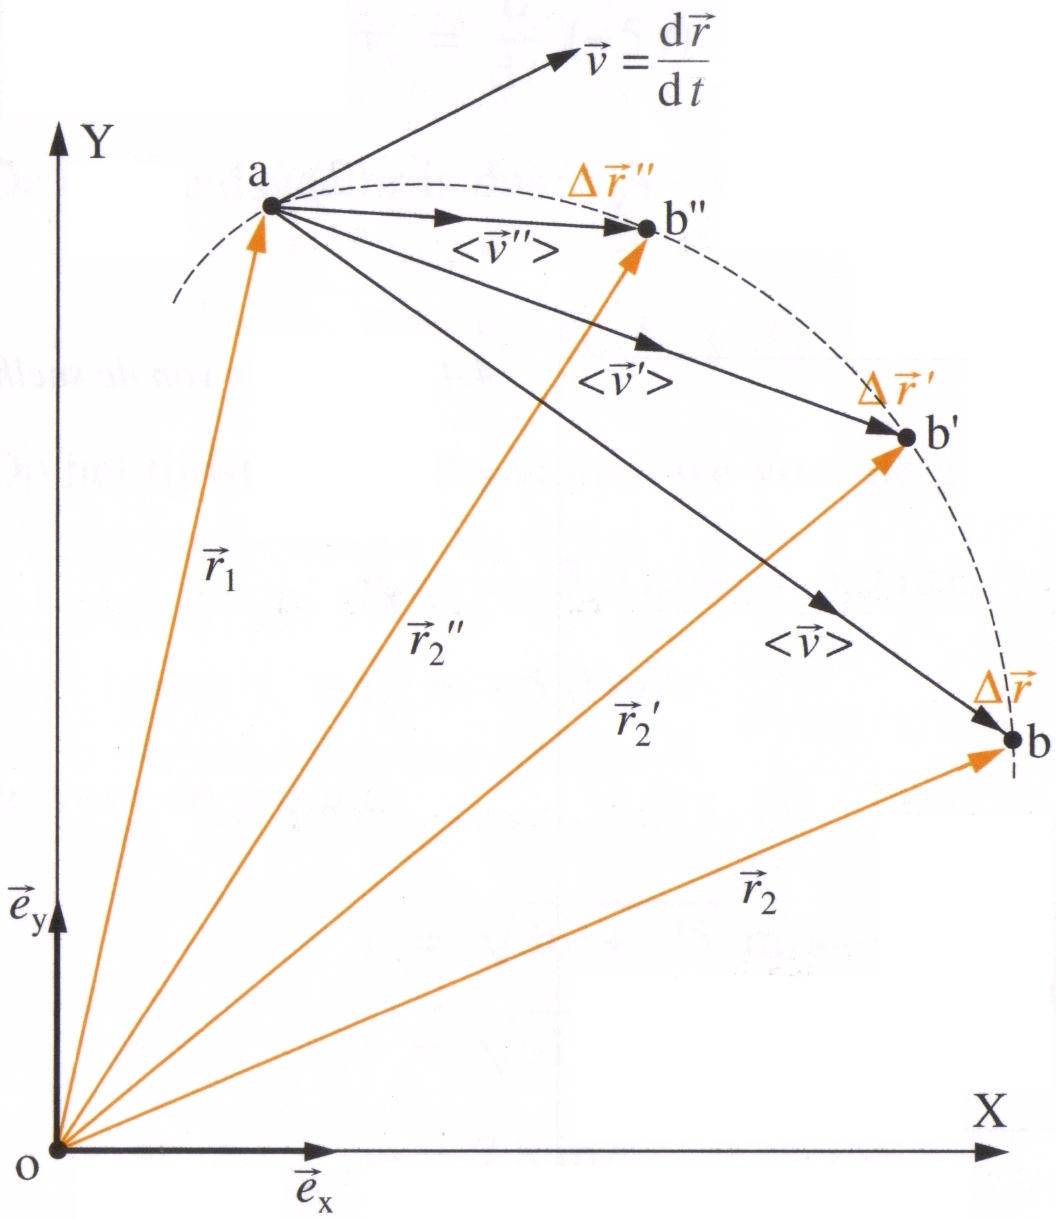
\includegraphics[width=0.38\textwidth]{gem_snelheidsvector}
%%\hspace{1cm}
%\includegraphics[width=0.4\textwidth]{snelheidsvector}
%\caption{De snelheidsvector is te ontbinden in componenten}
%\end{figure}
%\newline

\newpage

\begin{eigenschap}
De snelheidsvector is rakend aan de baan.
\end{eigenschap}
%\begin{figure}[h]
%\centering
%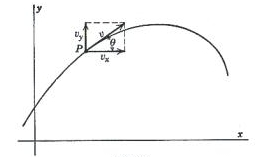
\includegraphics[width=0.4\textwidth]{snelheidrakend}
%\caption{De snelheid raakt aan de baan}
%\end{figure}
\begin{proof}
We kunnen dit bewijzen met de kettingregel, toegepast op de functie $y(t)=y(x(t))$.
\begin{eqnarray*}
 \frac{dy}{dt}=\frac{dy}{dx}\frac{dx}{dt}\Leftrightarrow\frac{dy}{dx}=\frac{\frac{dy}{dt}}{\frac{dx}{dt}}=\frac{v_y}{v_x}
\end{eqnarray*}
Inderdaad, $\frac{dy}{dx}$ is de helling van de baan en deze valt samen met de helling die de snelheidsvector maakt $\frac{v_y}{v_x}$.
\end{proof}

\subsection{Versnelling}

Ook de versnelling definieren we analoog; als afgeleide van de snelheid.
\begin{eqnarray*}
\vec{a}=\frac{d\vec{v}}{dt}=\frac{dv_x}{dt}\vec{e}_x+\frac{dv_y}{dt}\vec{e}_y=a_x\vec{e}_x+a_y\vec{e}_y
\end{eqnarray*}
Merk op dat er een versnelling kan zijn wanneer de snelheidsvector van grootte verandert maar \'o\'ok wanneer de snelheidsvector van richting verandert! Als de snelheidsvector immers van richting verandert, veranderen zijn co\"ordinaten $v_x$ en/of $v_y$. Merk bovendien op dat de versnelling niet noodzakelijk samen hoeft te vallen met de baan \ldots
\begin{figure}[h]
\centering
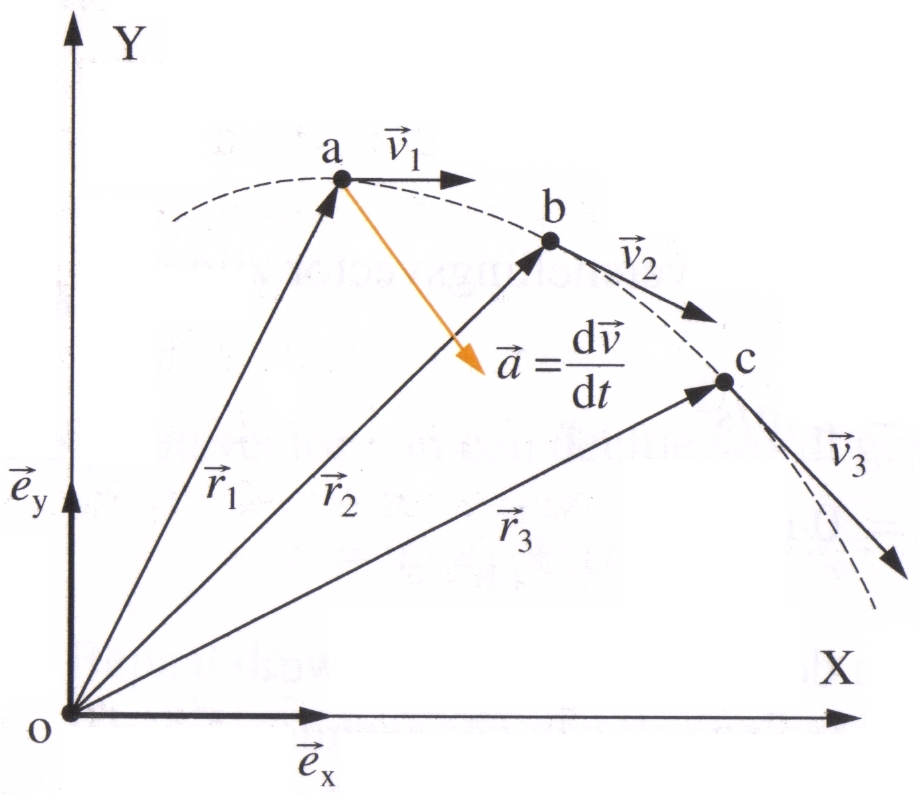
\includegraphics[width=0.4\textwidth]{versnellingsvector}
\caption{De versnelling raakt niet noodzakelijk aan de baan}
\end{figure}

\newpage

%oefening baanvergelijking, enz.

\begin{enumerate}
\item[\textbf{Opdracht}]\textsf{De positie van een deeltje als functie van de tijd wordt beschreven door
\begin{displaymath}
\vec{r}=bt\vec{e}_x+(c-dt^2)\vec{e}_y
\end{displaymath}
met $b=2,00\rm\,m/s$, $c=5,00\rm\,m$ en $d=1,00\rm\,m/s^2$.
\begin{enumerate}
\item Druk $y$ uit in functie van $x$. Hoe ziet de baan eruit?
\item Bepaal de snelheidsvector.
\item Op welk tijdstip ($t>0$) staat de snelheid loodrecht op de plaatsvector?
\end{enumerate}
\item[\textit{oplossing}]
\begin{enumerate}
\item We moeten dus de baanvergelijking geven. Dit doen we door de tijd uit te drukken i.f.v. de positie $x$ en dit te substitueren in de co\"ordinaatvergelijking $y(t)$.
\begin{eqnarray*}
x&=&bt\Leftrightarrow t=\frac{x}{b}\\
&\Downarrow&\\
y&=&c-dt^2=c-\frac{d}{b^2}x^2
\end{eqnarray*}
Dit is een bergparabool met top $(0,c)=(0,5,00\rm\,m)$
\item De componenten van de snelheid zijn:
\begin{eqnarray*}
v_x&=&\frac{dx}{dt}=b\\
v_y&=&\frac{dy}{dt}=-2dt
\end{eqnarray*}
zodat de snelheid(svector) wordt gegeven door
\begin{eqnarray*}
\vec{v}&=&v_x\vec{e}_x+v_y\vec{e}_y\\
&=&b\vec{e}_x-2dt\vec{e}_y
\end{eqnarray*}
\item De rechte die de richting van de snelheid weergeeft, staat loodrecht op de rechte die de richting van de positievector weergeeft wanneer het product van de richtingsco\"effici\"enten gelijk is aan $-1$:
\begin{eqnarray*}
rc_{r}\cdot rc_{v}&=&-1\\
&\Updownarrow&\\
\frac{y}{x}\cdot\frac{v_y}{v_x}&=&-1\\
&\Downarrow&\\
\frac{c-dt^2}{bt}\cdot\frac{-2dt}{b}&=&-1\\
&\Downarrow&(t>0)\\
t&=&\sqrt{\frac{2cd-b^2}{2d^2}}\\
&=&1,73\rm\,s
\end{eqnarray*}
\end{enumerate}}
\end{enumerate}

\newpage

\section{De eenparige cirkelbeweging}

De cirkelbeweging is op het eerste zicht misschien een zeer eenvoudige beweging maar wel alom tegenwoordig. Denk maar aan een tolbeweging, een kermisattractie zoals een carrousel, wielen, planeetbanen of aan het nemen van een bocht met de auto of de fiets. Vandaar dat het een toch een erg belangrijke beweging is. Wij bestuderen een eenparige cirkelbeweging (ECB). Dat betekent dat de baan van het object een cirkel is en dat de grootte van de snelheid waarmee de baan wordt doorlopen, constant is.

\subsection{Enkele begrippen}

Om een cirkelbeweging te beschrijven, hebben we enkele begrippen nodig die je eventueel nog onbekend zijn. Zo is er de \emph{frequentie}. Het is algemeen het aantal trillingen of cyclussen van een periodieke beweging die per seconde worden doorlopen. Specifiek voor de cirkelbeweging is de frequentie dan het aantal keren dat de cirkel doorlopen wordt per tijdseenheid. De frequentie krijgt het symbool $f$ en heeft als eenheid de Hertz, $[f]=\rm Hz=s^{-1}$. Het begrip \emph{periode} gebruiken we voor de tijdsduur die nodig is voor het doorlopen van \'e\'en cyclus. Het symbool is $T$ en de eenheid seconde, $[T]=s$. Het aantal cyclussen dat in de periode wordt doorlopen is \'e\'en zodat de volgende relatie tussen de frequentie en de periode bestaat.
\begin{equation*}
f=\frac{1}{T}
\end{equation*}
Als laatste hebben we nog het begrip \emph{hoeksnelheid}. 
\begin{figure}[h]
\centering 
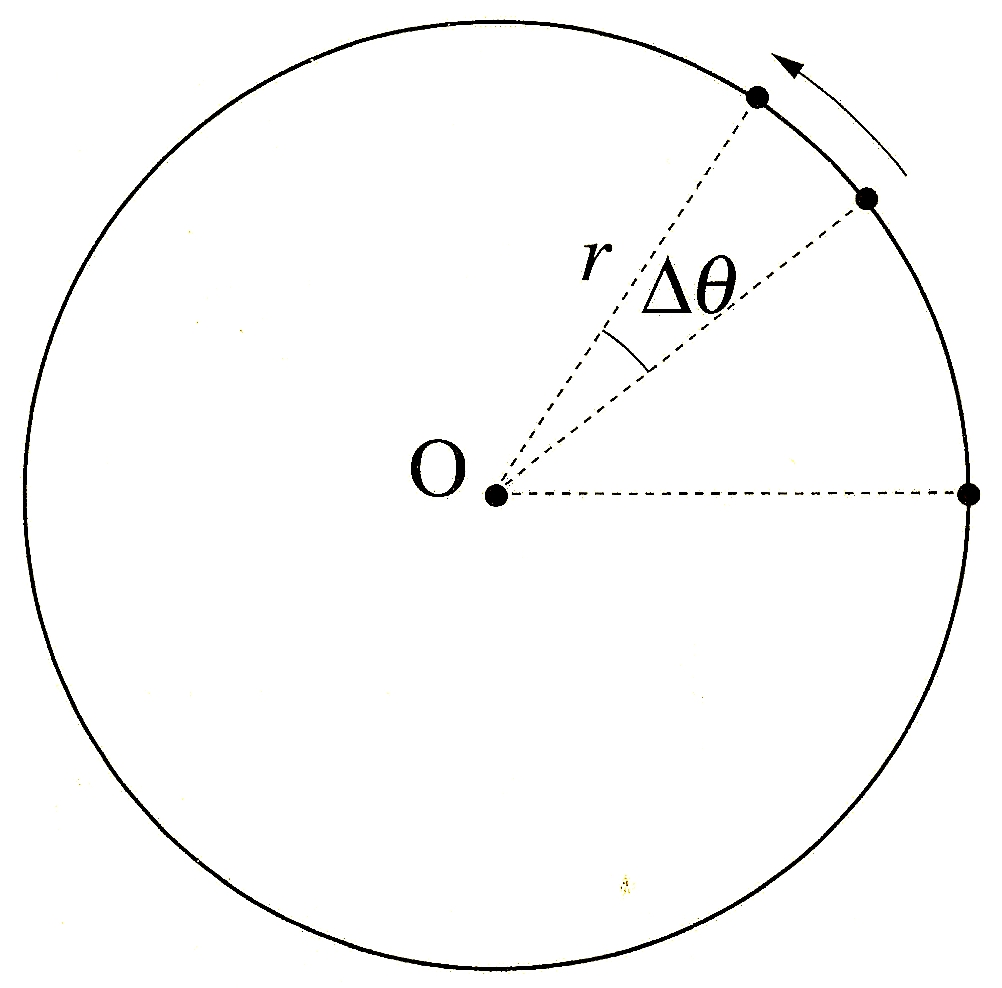
\includegraphics[width=0.35\textwidth]{ecb_hoeksnelheid}
\caption{De hoeksnelheid}
 % ecb_hoeksnelheid.jpg: 1002x988 pixel, 72dpi, 35.35x34.85 cm, bb=0 0 1002 988
\end{figure}
Verschillende punten op je fietswiel hebben verschillende snelheden als hun afstand tot het centrum verschilt. Het ventieldopje moet immers in eenzelfde tijd meer afstand afleggen dat het sensortje van je snelheidsmeter. Toch bestaat het wiel uit \'e\'en geheel. Als je naar de omwentelingshoek kijkt die een straal vanuit het centrum door een punt op het wile maakt, dan is die voor alle punten gelijk. Hoe sneller het wiel draait, hoe groter ook de omwentelingshoek is die een straal gemaakt heeft. Daarom defini\"eren we de hoeksnelheid $\omega$ als de verandering van de omwentelingshoek tot de benodigde tijd.\footnote{De letter $\omega$ is de kleine letter van $\Omega$ en de laatste letter in het Griekse alfabet. Spreek $\omega$ uit als omega. Een $\omega$ is geen w, zoals ook een w geen $\omega$ is. O wee ($\omega$?) als je je op het examen in juni vergist \ldots}
\begin{equation*}
\omega=\frac{\Delta\theta}{\Delta t}
\end{equation*}
De eeneid is radialen per seconde, $[\omega]=\rm rad/s$. Aangezien een volledige omwentelingshoek $2\pi$ bedraagt en de tijd nodig om rond te gaan de periode is, geldt
\begin{equation}
\omega=\frac{2\pi}{T}=2\pi f\label{hoeksnelheid}
\end{equation}

\subsection{Kinematica van de cirkelbeweging}

We beschouwen een punt dat een cirkelbeweging maakt met straal $r$. We voeren een assenstelsel in met de oorsprong in het middelpunt van de cirkel. 
\begin{figure}[h]
\centering
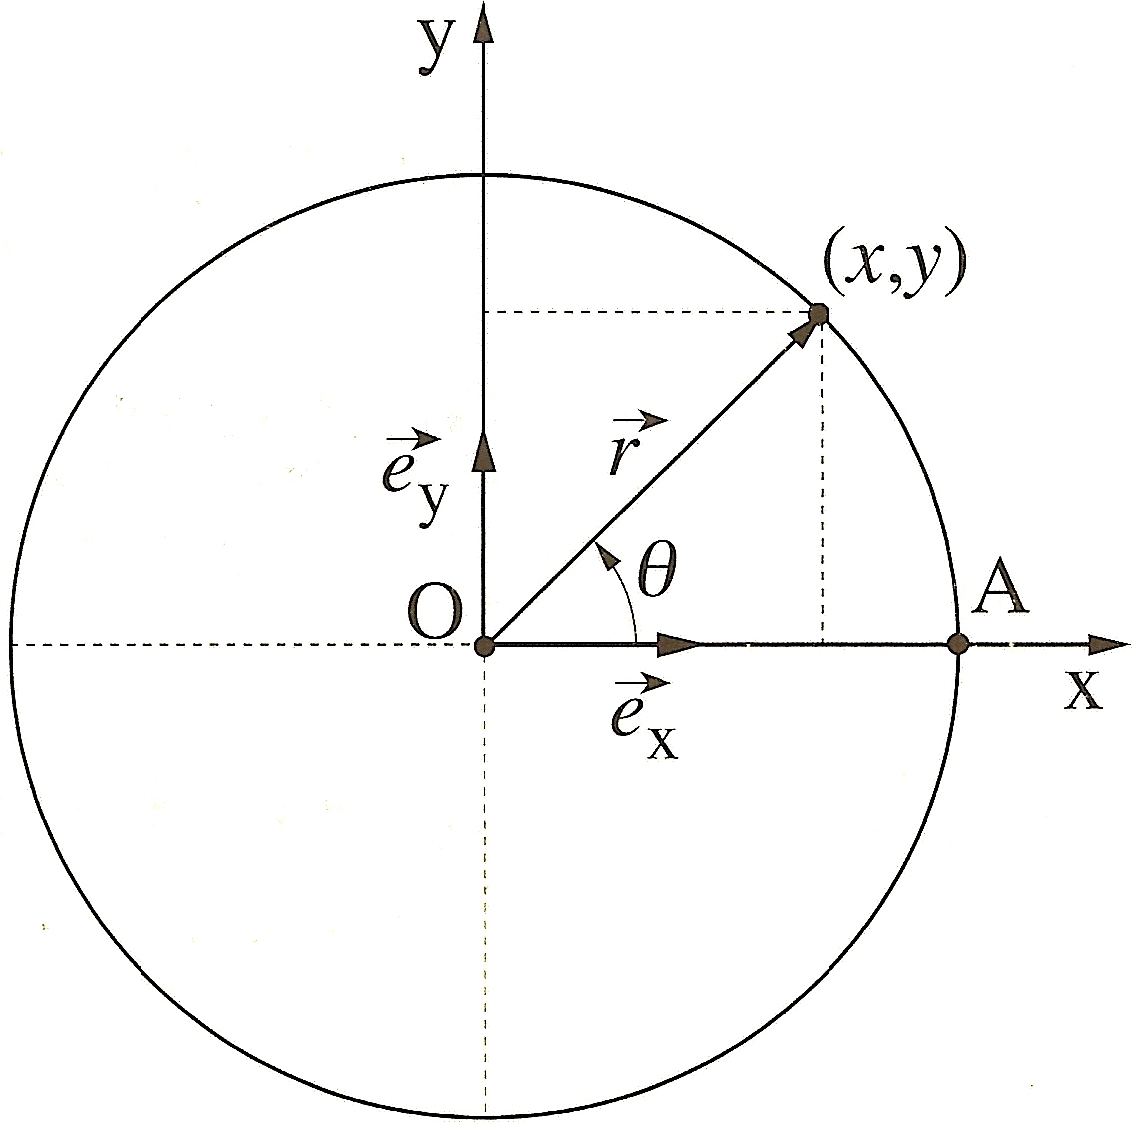
\includegraphics[width=0.4\textwidth]{ecb_positie}
\caption{Co\"ordinaten}
\end{figure}
Als we de omwentelingshoek $\theta$ meten vanaf de positieve $x$-as en en het tijdstip $t_0=0$ nemen, kunnen we de doorlopen omwentelingshoek als volgt in functie van de tijd schrijven.
\begin{equation*}
\omega=\frac{\Delta\theta}{\Delta t}=\frac{\theta-\theta_0}{t-t_0}=\frac{\theta}{t}\quad\Rightarrow\quad\theta=\omega t
\end{equation*}
De co\"ordinaatfuncties vinden we dan als projecties op de $x$- en $y$-as.
\begin{eqnarray*}
x(t)&=&r\cos\omega t\\
y(t)&=&r\sin\omega t
\end{eqnarray*}
We krijgen dan voor de plaatsvector, de snelheid en de versnelling:
\begin{eqnarray}
\vec{r}&=&r\cos\omega t\cdot\vec{e}_x+r\sin\omega t\cdot\vec{e}_y\nonumber\\
&\Downarrow&
\left\{\begin{array}{l}
v_x=\frac{dx}{dt}=-\omega r\sin\omega t\\
v_y=\frac{dy}{dt}=\omega r\cos\omega t
\end{array}
\right.\nonumber\\
\vec{v}&=&-\omega r\sin\omega t\cdot\vec{e}_x+\omega r\cos\omega t\cdot\vec{e}_y\nonumber\\
&\Downarrow&
\left\{\begin{array}{l}
a_x=\frac{dv_x}{dt}=-\omega^2 r\cos\omega t\\
a_y=\frac{dv_y}{dt}=-\omega^2 r\sin\omega t
\end{array}
\right.\nonumber\\
\vec{a}&=&-\omega^2 r\cos\omega t\cdot\vec{e}_x-\omega^2 r\sin\omega t\cdot\vec{e}_y\nonumber\\
&=&-\omega^2(r\cos\omega t\cdot\vec{e}_x+r\sin\omega t\cdot\vec{e}_y)\nonumber\\
&\Updownarrow&\nonumber\\
\vec{a}&=&-\omega^2\vec{r}\label{versnelling}
\end{eqnarray}
Deze laatste gelijkheid is erg belangrijk. We vinden dat de versnelling steeds naar het middelpunt van de cirkel is ge\"ori\"enteerd \ldots! We noemen het bijgevolg een centripetale\footnote{Dit is niet hetzelfde als centrifugaal.} of middelpuntzoekende versnelling. 
\begin{figure}[h]
\centering
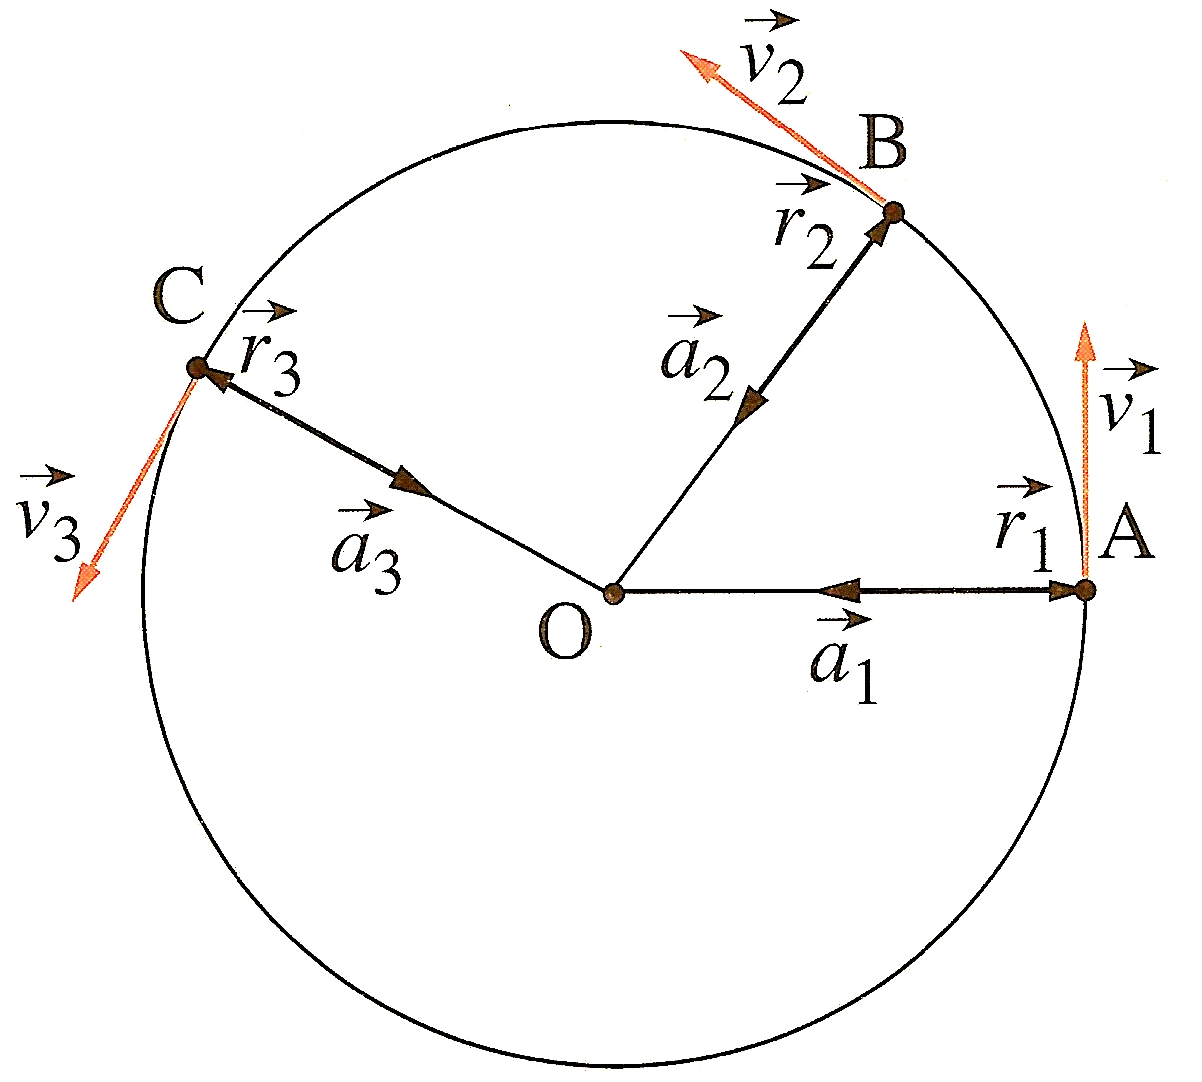
\includegraphics[width=0.4\textwidth]{ecb_versnelling}
\caption{De middelpuntzoekende versnelling}
\end{figure}
Je zou dit resultaat opmerkelijk kunnen noemen aangezien de snelheid een constante grootte heeft.
\begin{eqnarray}
v=\parallel\vec{v}\parallel&=&\sqrt{v_x^2+v_y^2}\nonumber\\
&=&\sqrt{(-\omega r\sin\omega t)^2+(\omega r\cos\omega t)^2}\nonumber\\
&=&\sqrt{r^2\omega^2(\sin^2\omega t+\cos^2\omega t)}\nonumber\\
&\Updownarrow&\nonumber\\
v&=&r\omega\label{snelheid}
\end{eqnarray}
Echter verandert de richting van de snelheid en aangezien de versnelling de verandering van de snelheid is, moet er een versnelling zijn. Deze is naar het centrum ge\"ori\"enteerd omdat een fractie van een seconde later het object -- in vergelijking met de baan die het zou afleggen moest het volgens de snelheid die het op een bepaald moment heeft, voortbewegen -- iets dichter naar het centrum moet zijn gekomen. De snelheidsvector is in grootte niet veranderd maar wel gedraaid, in de richting van het centrum. Moest bovendien de versnelling niet loodrecht op de snelheid staan, dan zou de versnelling een component volgens de snelheid hebben wat zou betekenen dat de snelheid in die richting zou moeten toenemen.
\begin{figure}[h]
\centering
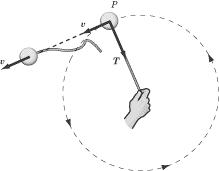
\includegraphics[width=0.4\textwidth]{ballnostring}
\caption{Moest er geen versnelling naar het centrum zijn -- bv. in het geval dat een touwtje met een ronddraaiend object aan, knapt -- dan zou de snelheid niet veranderen en het object op een rechte baan in het verlengde van de snelheid met een constante snelheid voortbewegen.}
\end{figure}

Uit (\ref{hoeksnelheid}), (\ref{versnelling}) en (\ref{snelheid}) vinden we nog:
\begin{equation}
a=r\omega^2=v\omega=\frac{v^2}{r}
\end{equation}
Merk op dat de snelheid een kwadratische invloed op de grootte van de versnelling heeft.

\newpage


\section{De horizontale worp}

We bekijken een voorbeeld van een tweedimensionale beweging. Wanneer een object horizontaal met een bepaalde beginsnelheid wordt gecatapulteerd, noemen we die beweging een horizontale worp. Wij beschouwen de worp in het luchtledige.
\begin{figure}[h]
\centering
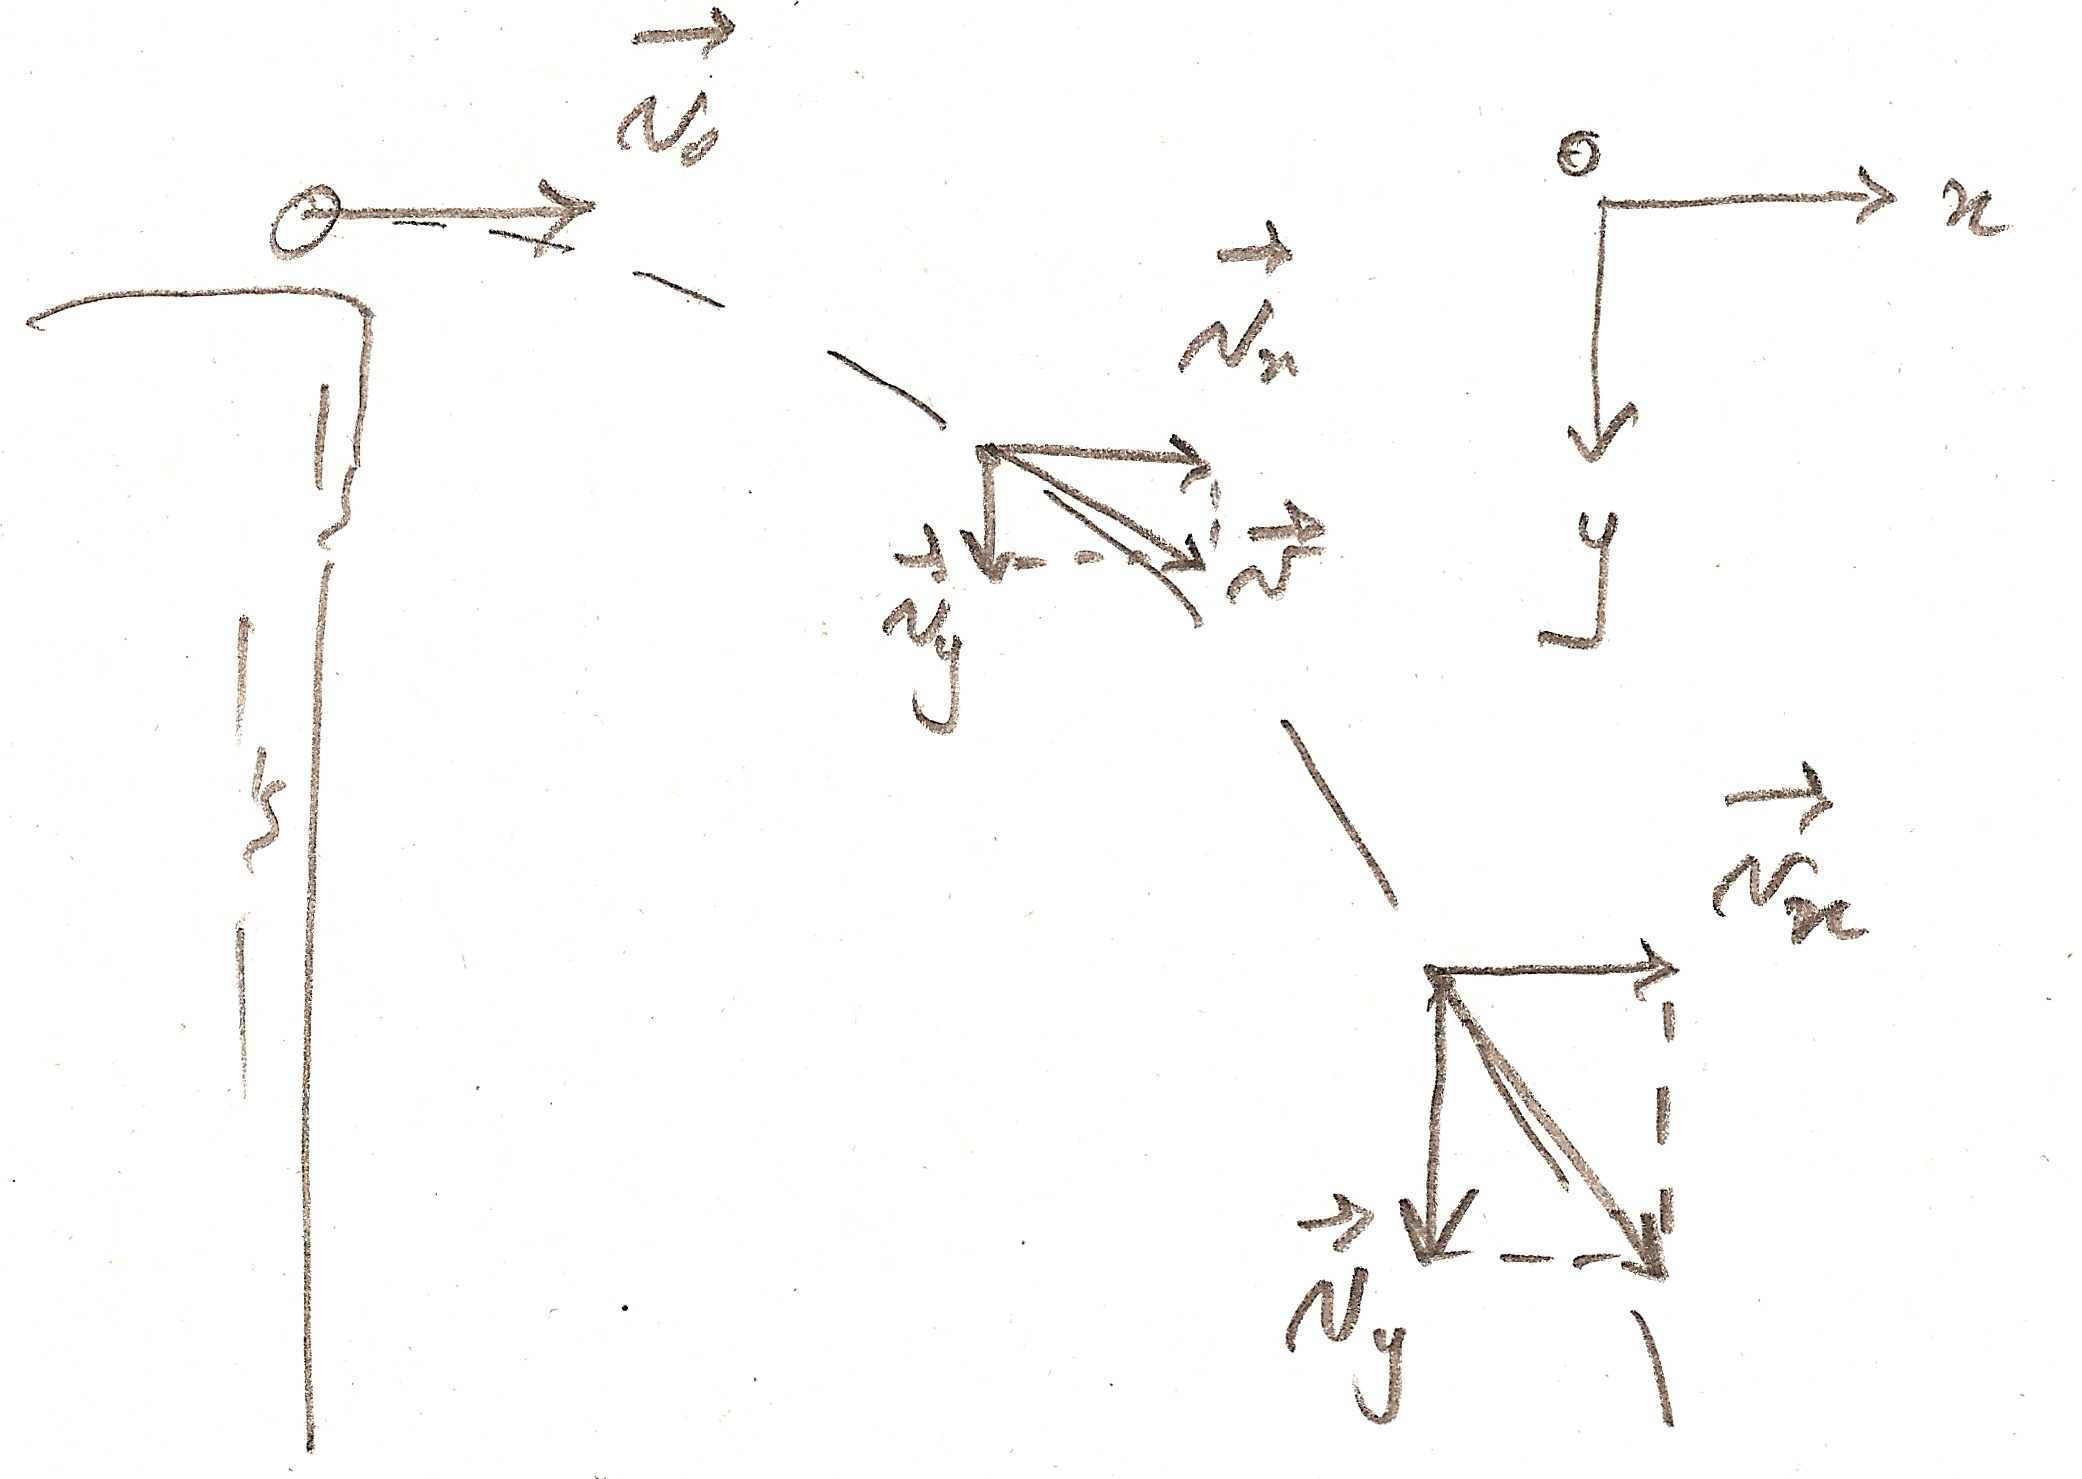
\includegraphics[width=0.6\textwidth]{horizontaleworp_tekening}
\caption{De snelheid in horizontale richting verandert niet, die in de verticale richting neemt lineair toe in de tijd}
\end{figure}
\newline
In de beschrijving kunnen we de $x$-as horizontaal en de $y$-as verticaal naar beneden nemen. Omdat er volgens de $x$-as geen versnelling is het lichaam volgens de $y$-as valt met de valversnelling $g$, kunnen we de formules voor een ERB en een EVRB (Zie (\ref{x(t)0}) en (\ref{v(t)0})) op de afzonderlijke assen toepassen en zo de volledige beweging beschrijven.%\footnote{Strikt genomen zoeken we hier nog niet naar een verklaring (die voor de horizontale beweging in de wet van de traagheid zit) maar beschrijven we enkel de beweging. Waarom de versnelling nul en $g$ is, vragen we ons dus zogezegd nog even niet af.}.
\begin{equation*}
\left\{
\begin{array}{l}
a_x=0\\
a_y=g
\end{array}
\right.
\Rightarrow
\left\{
\begin{array}{l}
v_x=v_0\\
v_y=gt
\end{array}
\right.
\Rightarrow
\left\{
\begin{array}{l}
x=v_0t\\
y=\frac{1}{2}gt^2
\end{array}
\right.
\end{equation*}
De baanvergelijking vinden we zoals eerder vermeld, door $t$ in functie van $x$ te schrijven $x=v_0t\Leftrightarrow t=\frac{x}{v_0}$ en dit in $y(t)$ te substitueren:
\begin{eqnarray*}
%&&x=v_0t\Leftrightarrow t=\frac{x}{v_0}\\
y=\frac{1}{2}gt^2=\frac{1}{2}g\left(\frac{x}{v_0}\right)^2=\frac{g}{2v_0^2}x^2
\end{eqnarray*}
De baan is dus een parabool.

\newpage

%oefening horizontale worp

\begin{enumerate}
\item[\textbf{Opdracht}]\textsf{Een vliegtuig vliegt met een snelheid van $450\rm\,km/h$ op een hoogte van $920\rm\,m$.
\begin{enumerate}
\item Hoever voor het doel moeten de voedselpakketten gelost worden
om op het doel terecht te komen?
\item Hoeveel tijd hebben de pakketten nodig om het doel te bereiken?
\end{enumerate}
\item[\textit{gegeven}]$v_0=125\rm\,m/s$\newline$y=920\rm\,m$
\item[\textit{gevraagd}]$x$, $t$
\item[\textit{oplossing}]De afstand waarover de voedselpakketten in
horizontale richting zijn vooruit gegaan, kunnen we vinden met de
baanvergelijking. We weten namelijk hoever de pakketten naar beneden
zijn gevallen en wat hun beginsnelheid is:
\begin{eqnarray*}
y&=&\frac{g}{2v_0^2}x^2\\
&\Downarrow&\\
x&=&v_0\sqrt{\frac{2y}{g}}=1712\rm\,m
\end{eqnarray*}
De valtijd voor de pakketten vinden we o.a. door naar de verticale
valbeweging te kijken. Deze gebeurt onafhankelijk van wat er in de
horizontale richting gebeurt, zodat:
\begin{eqnarray*}
y&=&\frac{1}{2}gt^2\\
&\Downarrow&\\
t&=&\sqrt{\frac{2y}{g}}=13,7\rm\,s
\end{eqnarray*}}
\end{enumerate}

\cleardoublepage
\newpage